\subsection{Redes neuronales artificiales}

\paragraph{}Una red neuronal artificial es un algoritmo o clasificador de aprendizaje automático, utilizada tanto para problemas de clasificación como de regresión.
Su concepción está inspirada en parte por la observación de los mecanismos de aprendizaje en sistemas biológicos. Las redes neuronales artificiales están formadas por unidades más simples e interconectadas, donde cada unidad tiene entradas reales y produce una única salida también real, mediante asignación de pesos en regresiones lineales.

\paragraph{}Los perceptrones son las unidades sobre las cuales están construidos los sistemas de redes neuronales, dado que por sí solos únicamente puede expresar decisiones lineales, pero su composición en redes neuronales multicapa puede expresar una variedad de funciones objetivo no lineales. Un perceptrón recibe valores de $n$ entradas $x_1, x_2, \dots x_n$, realiza una combinación lineal con ellas obteniendo una expresión $x_1 w_1 + x_2 w_2 + \dots x_n w_n$ donde $w_i$ es el peso otorgado a $x_i$, para todo $i \in \{1, \dots, n\}$. Esta expresión es evaluada con una función conocida como \textit{función de activación}, que devuelve un valor de acuerdo a si se supera un umbral determinado o no con la combinación lineal de los valores de entrada. Por ejemplo, si se utiliza a la función signo como función de activación, si la combinación lineal de los valores de entrada es mayor que cero, se devolverá $1$ como salida y $-1$ en caso contrario. La figura \ref{fig:perceptron} muestra la estructura de dicho perceptrón.

\textsc{\begin{figure}[ht!]
	\centering
    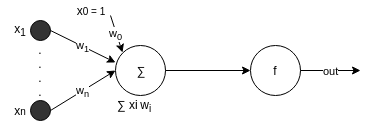
\includegraphics[width=.5\linewidth]{imagenes/perceptron.png}
	\caption{Perceptron con función de activación \textit{f = signo(x)}}
	\label{fig:perceptron}
\end{figure}}

\paragraph{}Cuando se calcula la combinación lineal de los valores de entrada, su valor resultante puede oscilar entre $-\infty$ y $+\infty$, dado que desde un perceptrón no se posee una referencia de cuáles son los límites presentes en las posibles clases de clasificación para el problema de interés, las funciones de actuvación se utilizan con el propósito de limitar este valor para producir la salida del preceptrón. El perceptrón puede ser utilizado para modelar funciones lógicas, como AND, OR, NAND y NOR, ajustando la cantidad de entradas según la cantidad de entradas de la función lógica y ajustando los pesos de tal menera que las salidas sean 1 y -1. El hecho de que los perceptrones puedan representar funciones lógicas es relevante puesto que da lugar a que cualquier función lógica pueda ser representada mediante una red de perceptrones de dos niveles de profundidad, en la cual las entradas son conectadas a multiples perceptrones y las salidas de estos son conectadas a las siguientes capas. En general es de interés el estudio de redes multicapa de unidades, dado que de esta manera se pueden representar grandes variedades de funciones.

\paragraph{}Los perceptrones son un tipo de unidades que pueden ser utilizados en la creación de redes multicapa. En particular, múltiples capas de perceptrones dada su naturaleza de unidades lineales, producirán funciones lineales. Lo que se requiere son unidades cuyas salidas sean funciones no lineales de sus entradas. Una alternativa viable es la \textit{unidad sigmoide} cuya estructura es similar a la del perceptrón, variando en la función de activación, utilizando la función \textit{sigmoide} que es una función no lineal diferenciable. 

\paragraph{}Dada la estructura de la unidad, el aprendizaje se traduce en el problema de encontrar un vector de pesos $(w_0,w_1,\dots,w_n)$ tal que haga que la salida de la unidad sea la esperada. Dado que en este trabajo se utilizan redes multicapa, se utiliza el algoritmo \textit{Backpropagation} para \textit{aprender} los vectores de pesos de una red que tiene una cantidad dada fija de unidades interconectadas. Antes de explicar la naturaleza de el algoritmo \textit{Backpropagation} y cómo este ajusta de manera iterativa los pesos de las unidades, es importante tener en cuenta el concepto de \textit{gradiante descendente}. \textit{Gradiante descendente} es una técnica que busca encontrar un mínimo de una función, ya sea local o no. La búsqueda por \textit{gradiante descendente} encuentra un vector de pesos que minimiza el error con respecto al hiperplano generado por los vectores de pesos asociados al conjunto de entrenamiento, comenzando por un vector de pesos inicial arbitrario, modificándolo en pequeños pasos, realizando cada modificación de tal manera que se produce una disminución en el error con respecto al hiperplano de pesos asociados a la solución. Este proceso continúa hasta que se llega a un error global mínimo. \textit{Gradiante descendente} es una estrategia de búsqueda en un espacio grande o infinito de hipótesis que se puede aplicar siempre que el espacio de hipótesis contenga hipótesis que pueden ser determinadas de forma paramétrica, como son los pesos en las unidades. Así también, se requiere que el error pueda ser diferenciado con respecto a estos parámetros. Esta estrategia tiene algunas dificultades fundamentales, una de ellas es que la velocidad de convergencia a un mínimo es lenta,pudiendo requerir varios miles de pasos para lograrla y además, si existen varios mínimos locales en la superficie de error no se garantiza que la búsqueda converga a un mínimo global.

\paragraph{}El algoritmo \textit{Backpropagation} es un método que se utiliza en redes multicapa para calcular el gradiante que se utiliza para el cálculo, utilizando \textit{gradiante descendete}, de los pesos de la red. El error es calculado en la salida de la red multicapa y el mismo es distribuído \textit{hacia atrás}, hacia las capas de la red, calculando para cada unidad perteneciente a una capa intermedia su error y actualizando sus pesos. El \textit{loop} de actualización de pesos en \texit{Backpropagation} puede iterar miles de veces en una aplicación típica de redes neuronales, por lo que existen una variedad de condiciones de parada como, detener el \textit{loop} luego de una cantidad fija de iteraciones o, detener el \textit{loop} luego de que el error pasa por debajo de cierto humbral definido o, por criterios definidos sobre un conjunto dado de prueba. Los criterios de terminación son importantes y su elección es delicada dado que de terminar antes de lo necesario con las iteraciones, la red neuronal puede devolver salidas con un error alto y, si se realizan muchas iteraciones se puede generar un sobreajuste de la red neuronal al conjunto de entrenamiento, produciendo resultados de bajo error para el conjunto de entrenamiento, pero con más altos niveles de error para conjuntos de prueba. \texit{Backpropagation} no asegura la convergencia a un mínimo global debido al uso \textit{gradiante descendente} en espacios de hipótesis de alta dimensionalidad, (pudiendo haber tantas dimensiones como pesos). Alta dimensionalidad incrementa la probabilidad de que los movimientos en la superficie de error no lleven a un mínimo global también pudiendo alcanzar mínimos para una o más dimensiones, que no son necesariamente mínimos para las otras dimensiones. A pesar de la falta de seguridad con respecto a la convergencia del algoritmo a un mínimo global, \textit{Backpropagation} es un método de aproximación de funciones altamente efectivo. Una propiedad importante este, es la habilidad de descubrir representaciones de los datos no tribiales en las capas intermedias escondidas de la red, generando así características intermedias más allá de los datos de entrada y la salida proporsionada por los datos de entrenamiento, reafirmando la capacidad de las redes neuronales de \textit{aprender} patrones en grandes cantidades de datos que no son aprendidos por otros métodos. 

\paragraph{}En este trabajo se construyen varios tipos de redes que varían en las funciones de activación que usan las unidades, a continuación se presentan las funciones de activación que se usaron durante este trabajo. La función \textit{tanh()}, expresada de la siguiente manera: $f(x) = tanh(x) = \frac{2}{1 + e^{-2x}} - 1 $ es una función continua no lineal y al componerla consigo misma se obtienen funciones no lineales, lo que permite combinar a unidades con esta función de activación sin perder la no linealidad. Es una función suave en su curva, mostrando que pequeñas variaciones en valores del dominio cercanos a 0 generan cambios grandes en los valores correspondientes del codominio; esto implica que se le da una gran ponderación a los valores de los extremos del codominio, algo análogo a una tasa de aprendizaje. La función \textit{relu()}, expresada de la siguiente manera: $f(x) = relu(x) = max(0, x)$ es no lineal y las composiciones de ella consigo misma serán no lineales, pero por su forma, puede generar que algunas neuronas den como resultado cero, constituyéndose una eventual pérdida de información. Este problema se llama \textit{dying relu problem}. Así también, computar relu es menos costoso que computar tanh porque implica operaciones matemáticas más simples. La función identity, también llamada de activación lineal, expresada de la siguiente manera: $f(x) = identity(x) = x$, siempre retorna el mismo valor que recibe en su argumento, lo que implica que equivale a una regresión lineal utilizando los pesos de la unidad.

% Ventajas y desventajas
\paragraph{}Entre las ventajas de utilizar redes neuronales se encuentran el hecho de que se adecuan correctamente a problemas en los cuales los datos de entrenamiento contienen ruido y en contextos en los cuales tiempos largos de entrenamiento son aceptables. Además, suelen mantener tiempos bajos en clasificación.
Además, como se menciona en la sección \ref{section-trabajos-tecnicas-clasificacion}, una desventaja de las redes neuronales es que su representación interna es difícil de entender para los humanos y por este motivo se dice que se comportan como una “caja negra”.